\documentclass{article}

% Language setting
% Replace `english' with e.g. `spanish' to change the document language
\usepackage[english]{babel}

% Set page size and margins
% Replace `letterpaper' with `a4paper' for UK/EU standard size
\usepackage[a4paper,top=2cm,bottom=2cm,left=3cm,right=3cm,marginparwidth=1.75cm]{geometry}

% Useful packages
\usepackage{amsmath}
\usepackage{graphicx}
\usepackage[colorlinks=true, allcolors=blue]{hyperref}
\usepackage{tabularx}
\usepackage{booktabs}
\usepackage{hyperref}
\usepackage[colorlinks=true,allcolors=blue]{hyperref}
\usepackage{float}
\usepackage{glossaries}
\usepackage{biblatex}
\usepackage{xcolor}
\usepackage[utf8]{inputenc}
\addbibresource{references.bib}
\makeglossaries

\newglossaryentry{IETF}{
name=IETF,
description={Internet Engineering Task Force, It's an organisation for further developing the internet}
}

\newglossaryentry{W3C}{
name=W3C,
description={World Wide Web Consortium, They develop standards and guidelines for the web}
}

\newglossaryentry{Zcash protocol}{
name=Zcash protocol,
description={privacy focused cryptocurrency that uses a protocol named zk-SNARKs}
}

\newglossaryentry{BBS}{
name=BBS,
description={short term use of BBS signature scheme}
}

\title{BBS Signature Scheme: From Theory to Implementation}
\author{Joel Gabriel Robles Gasser \& Miguel Angel Schweizer\\[1cm]{\small Advisors: Prof. Dr. Reto Koenig \& Prof. Dr. Rolf Haenni}}

\begin{document}
\maketitle

\begin{abstract}
This document is a documentation of the module BTI3041 Project 2 from the Berner Fachhochschule. The goal of this project is to implement a Java library for \gls{BBS}. 
It provides an in-depth overview of the BBS (Boneh-Boyen-Shacham) signature scheme, which is a secure multi-message digital signature protocol. It's core feature lies in the capability to sign a series of messages while generating a single, fixed-size digital signature. Furthermore, the holder of the BBS signature can generate a zero-knowledge proof, where these proofs demonstrate knowledge of the signature and allow for selective disclosure of the signed messages. There is no reveal of any information of the undisclosed messages and uphold the authenticity and integrity of the disclosed messages.  \newline

Before delving into the details of the BBS signature scheme, it is important to note that this document focuses specifically on the unique properties and functionalities of the signature scheme, furthermore it targets an audience with a basic foundation of cryptography. The foundational concepts of digital signatures and elliptic curve cryptography is not the focus of this document and are a requirement for the understanding of the BBS signature scheme. \cite{bbs-signature-identity}
\end{abstract}
\clearpage

\tableofcontents

\clearpage


\section{Introduction}
This document serves as an introduction to the Boneh-Boyen-Shacham(BBS) signature scheme, a keystone in the field of cryptographic protocols. The core task is to make a Java library for using the BBS signature scheme in applications. The \gls{IETF} BBS signature scheme draft \cite{bbs-signature-identity} provides a pseudo code for implementing \gls{BBS}. The main goal was to have a code that suits the pseudo code perfectly. The implemented code is written line by line like the pseudo code of the \gls{IETF} draft. Breaking down the BBS signature scheme and seeing what a wide comprehension is needed to understand all core principles of this cryptographic protocol was a challenge. Some sub-tasks were understand the elliptic curves perfectly, understand what pairings are, understand the BLS12-381 curve with it's calculations in \(G_1\) and \(G_2\). \\
Having it's principles of asymmetric cryptography, this scheme utilizes a pair of keys - a private key for signing messages and a corresponding public key for verifying these signatures. The BBS signature scheme is named after his creators Dan Boneh, Xavier Boyen and Hovav Shacham. This scheme extends beyond the basic functionalities of digital signatures to offer several distinct and advanced features. \cite{bbs-signature-identity}

\section{Tasks}

\subsection{Main Goal}
Before beginning the Project 2 module we already set the topic with our professors. We know what we wanted to do for our Bachelor thesis but did not really knew what specific topic we wanted to research and what our product would be for the Project 2 module. After explaining our ideas to Prof. Dr. Rolf Haenni, he gave us the idea to look into the BBS signature scheme, as it is a signature scheme that is new and barely applied in today's cryptography. We researched about the BBS signature scheme and chose it to be our topic for the Project 2 module. \\
We still didn't knew what our final product would be, so we found the IETF draft with the pseudo code for implementing the BBS signature scheme. After discussing our goal to implement the BBS signature scheme we still had to choose in which programming language we wanted to program it. Implementing it in C would be nice. But this idea was extremely fast discarded as it was easier to do the implementation in a language we are more than familiar with, Java.
So we set our main task to make a BBS signature scheme library in Java for using it in our bachelor thesis using the IETF draft as a recipe. It had to be as similar as possible to the draft line by line. \\
We didn't had the basics to understand the BBS signature scheme completely, so we made sub-tasks.

\subsection{Sub-tasks}
For understand the BBS signature scheme we first had to refresh our knowledge about elliptic curves and standard cryptographic primitives. Despite that we had to make sure what the features of \gls{BBS} was and what primitives it has.
First, we made a research about the features of \gls{BBS} and what the purpose of the signature scheme was. After having the top level, we moved on to the elliptic curves, this being the BLS12-381 curve with the topic of pairings. Explanations from our professors were needed to  completely understand all the topics. The pairings were to advanced to understand the mathematics behind it, so we only learned what they to and what their purpose was. 


\section{Key Features of BBS}

\subsection{Self-Sovereign Identity}

Self-sovereign identity is a model for managing digital identities. In this model the core concept is that individuals or corporations have the complete ownership and control of their accounts and personal data.

\subsection{Verifiable Credentials}

Verifiable credentials, also known as VC, are a \gls{W3C} standard for digital, cryptographically verifiable credentials. The VCs are stored on digital devices and use cryptography to verify the data and the authorship of the credentials. \cite{bbs-verifiable-credentials-blog}

\subsection{Trust Triangle}

\begin{figure}[H]
    \centering
    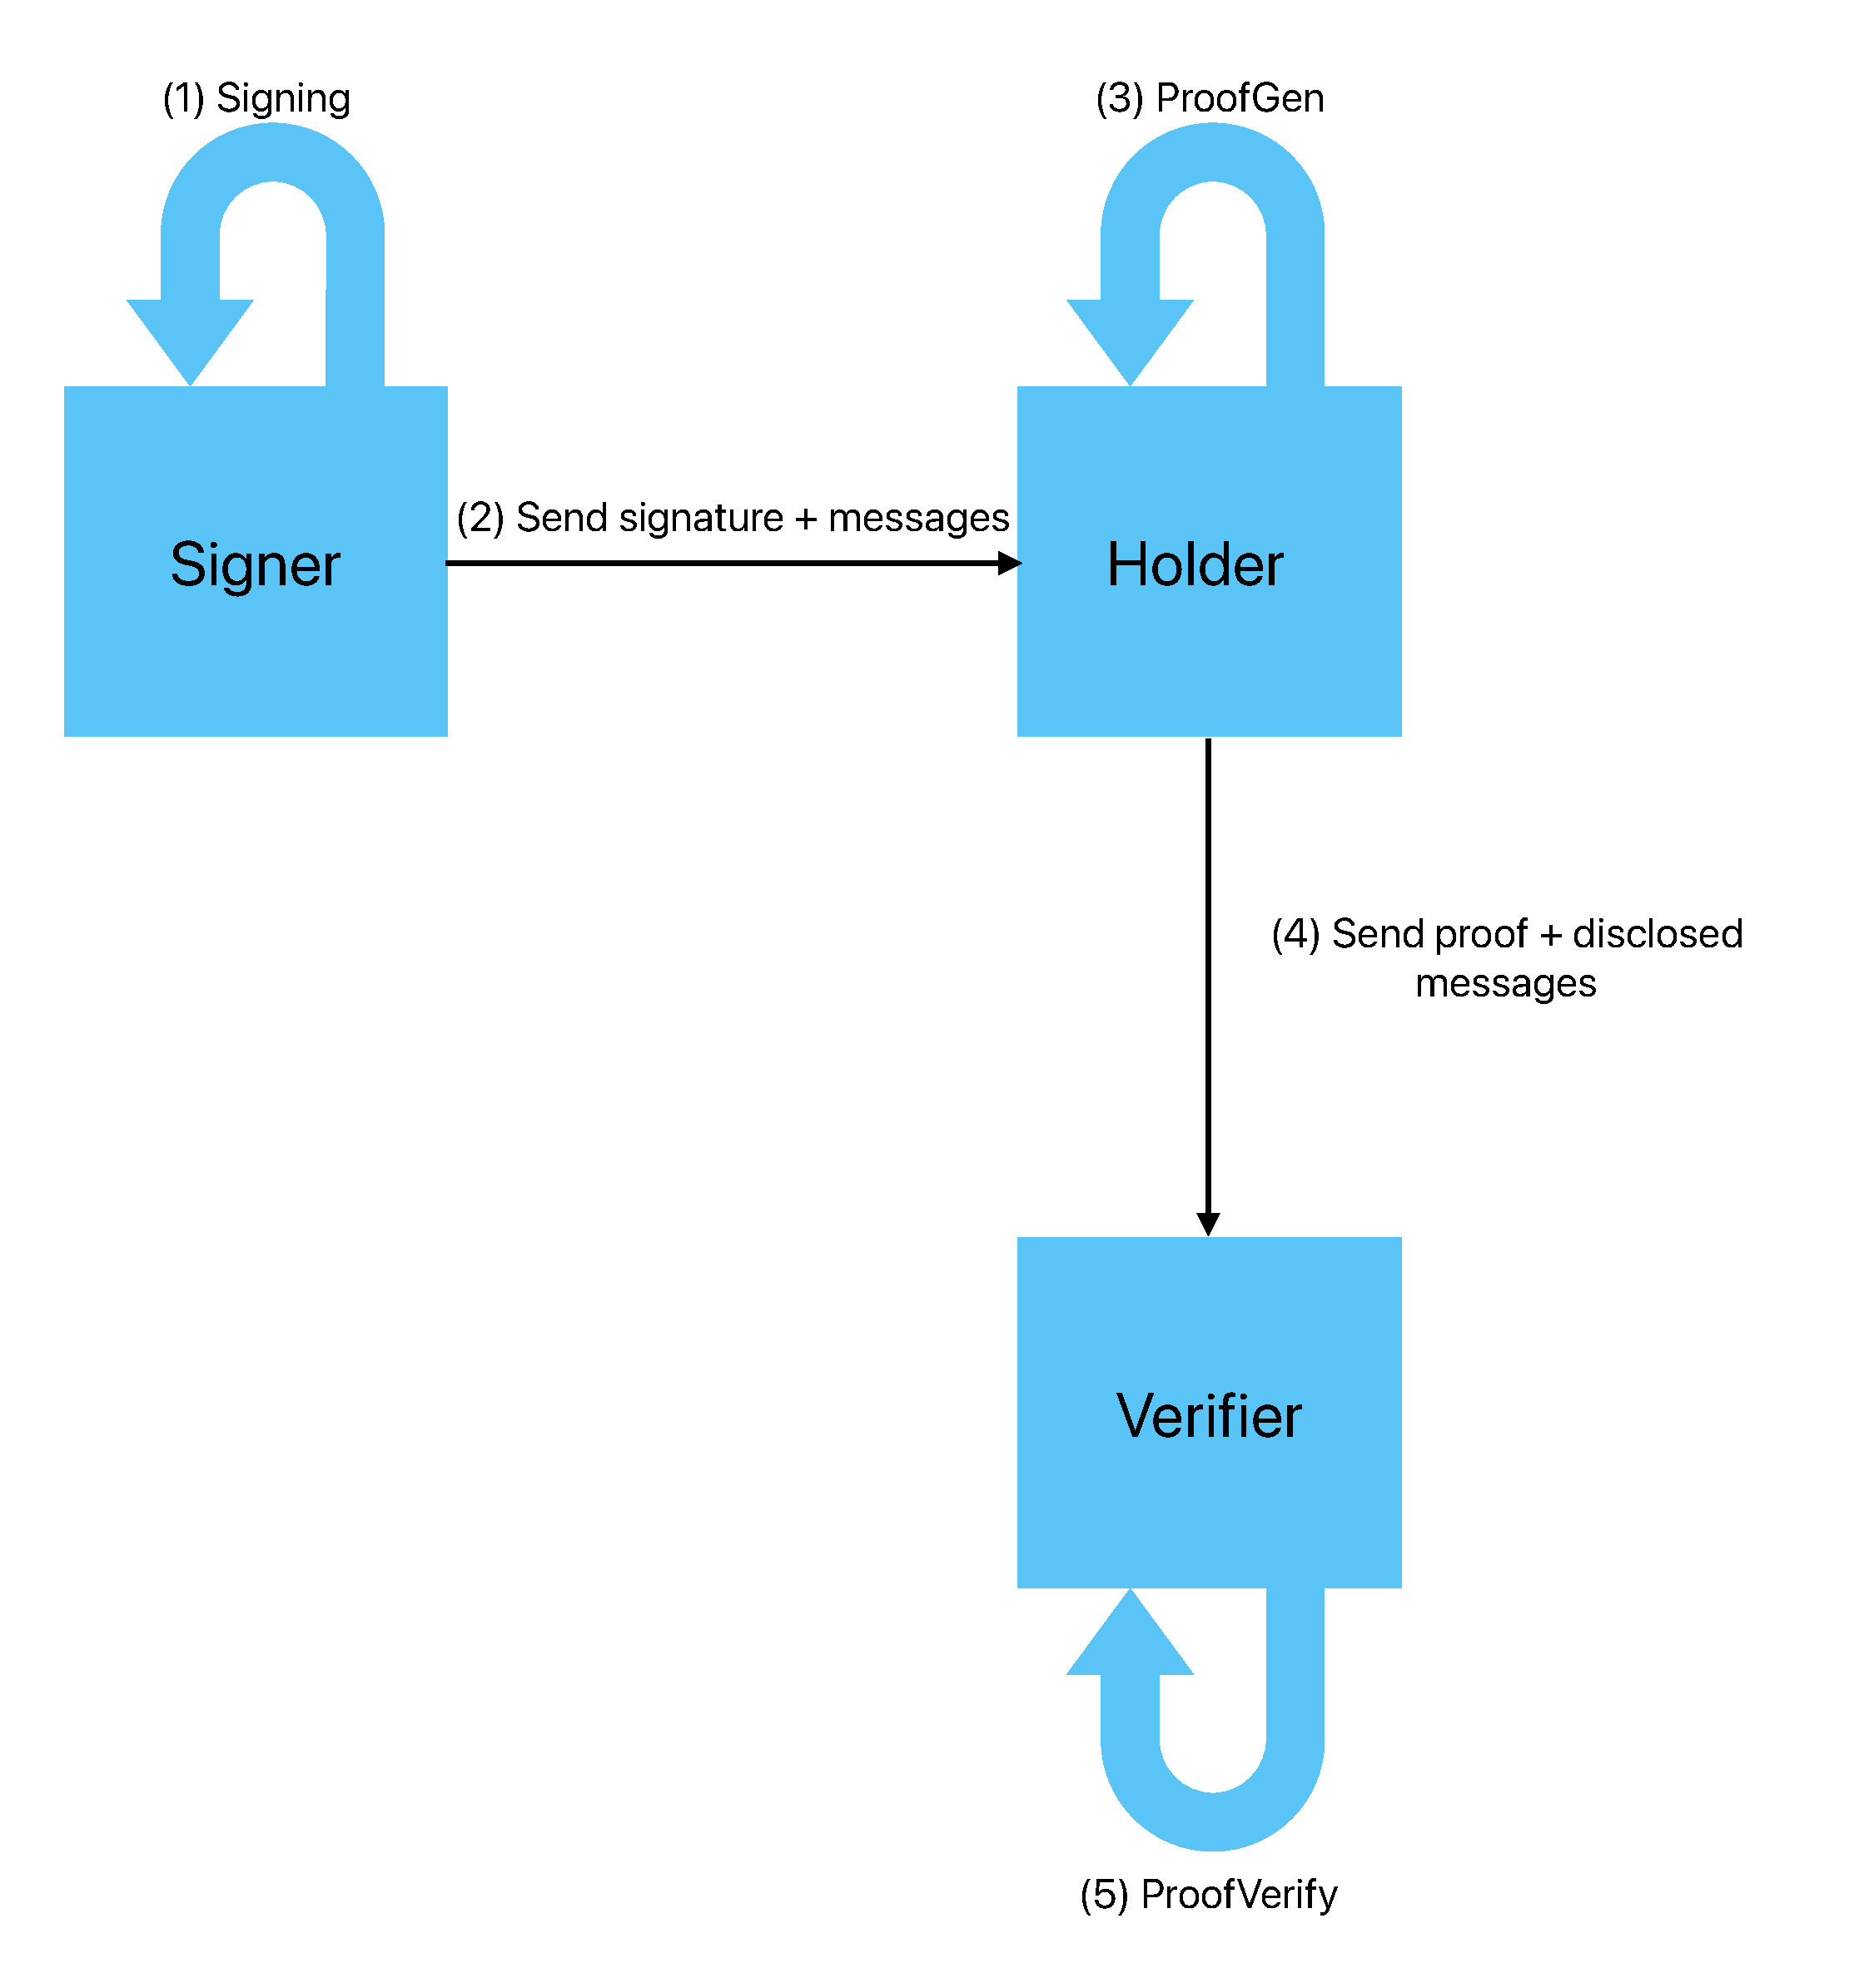
\includegraphics[width=0.5\linewidth]{diagram_entities.pdf}
    \caption{Diagram of main entities}
    \label{Fig: Diagram of the main entities}
\end{figure}

The trust triangle is a very important model for the BBS signature scheme, which provides the characteristics to the scheme and make the whole thing work between the parties. 
We have three-way relationship between parties which are signer, holder and verifier. The holder trusts the signer because he sends him his messages to be signed. 
The verifier trust the signer because he signed the messages of the holder. That is how the triangle of trust works. 

\subsubsection{Signer}
The signer is the party which signs and sends the messages from the holder and sends them back to the holder.

\subsubsection{Holder}
The holder makes a proof generation of the signature and the messages. He sends the messages he wants to have signed to the verifier. He also sends his generated proof and the disclosed messages to the verifier.

\subsubsection{Verifier}
The verifier verifies the proof he receives from the holder.



\subsection{Proof Of Knowledge \& Zero Knowledge Proof}

A lower version of zero-knowledge proof is the proof-of-knowledge. Proof-of-knowledge has the two characteristics of Completeness and Soundness. Completeness means that if the proof is true, the verifier can be convinced by the holder that they possess knowledge about the correct proof. Soundness is the opposite of completeness, if the proof is false, then no holder can convince a verifier that they possess knowledge about the proof. Zero-knowledge proof adds a characteristic known as zero-knowledge. This says that if a proof is true, then the verifier learns nothing more from the holder other than the proof is true. \cite{zero-knowledge-proofs}


\section{Properties of BBS}

\subsection{Selective Disclosure}

With BBS signature scheme we can sign multiple messages and produce a single output signature. This allows the holder to generate a proof of the messages and the signature. The holder itself can choose which message he wants to disclose, while revealing no-information about the undisclosed messages . The proof is a guarantee of integrity and authenticity of the disclosed message. \cite{bbs-signature-identity}

\subsection{Unlinkable Proofs}

The holder generates a proof, which is known as a zero-knowledge proof. In our case this means that a verifier cannot determine which signature was used to generate the proof. This removes a common source of correlation. Each proof generated is indistinguishable from random even for two proofs generated from the same signature. \cite{bbs-signature-identity}

\subsection{Proof of Possession}

The proof of possession means that the proofs generated by the scheme of the holder prove tot a verifier that the holder was in possession of a signature without revealing the signature itself. With the BBS signature scheme supports the binding of headers to the generated proof and hold additional information. \cite{bbs-signature-identity}

\subsection{Link Secrets}

Link secret enables more trusted interactions with verifiable credentials. With a cryptographic commitment algorithm the holder creates a commitment, which allows the holder to prove it knows the secret without revealing it. The holder can send the commitment to the signer, which signs it together with the credential attributes, while the secret is never shared. The link secret is a large random number. 
It is called link secret, because the master secret is inserted and signed in different credentials. By adding it in every credential, it links the holder to the credentials and link the credentials to each other. The master secret is randomized by a blinding algorithm at every issuance of a credential. The blinded master secret is called linked secret. The master secret is kept secret at every time and is never revealed by the holder. Only the commitments and proofs of knowledge of the committed secret are shared. \\
In the last IETF draft, the linked secrets were not included but they are working on adding linked secrets to the \gls{BBS} draft.
\cite{bbs-signature-identity}

\section{Elliptic Curve Pairings}
Elliptic curve pairings is a cryptographic primitive with a huge importance in the cryptography in today's world. Elliptic curve pairings expand the the versatility and usage of elliptic curve-based protocols. In elliptic curves the pairing is done by a function \textit{e()}. The mathematics behind pairings is very advanced algebra and will not be discussed in this document. Firstly we need to repeat what elliptic curves are in a short term and then we take on bilinearity.

\subsection{Elliptic Curves}

In the ever-evolving landscape of cybersecurity, the need for safe encryption methods to safeguard digital communication and protect sensitive information has never been more critical than nowadays. At the forefront of this cryptographic revolution stands Elliptic Curve Cryptography (ECC), a powerful and elegant branch of mathematics that has become vital in modern cybersecurity. 
Elliptic curves are defined over a field \textit{K} and describes points in \(K^2\).

\subsection{Bilinearity}
For understanding what bilinearity means, first we have to understand linearity. For example a function \(f(x)\) is linear if it satisfies these two properties: \\
Additivity: \(f(x + y) = f(x) + f(y)\) \\
Homogeneity: \(f(cx) = f(x)^c\) , where c is a constant \\
That is linearity. Now we take a function \(B(x,y)\), defined on two vector spaces V and W. The function \(B\) is bilinear if, for any constant \(a\), \(b\) and vectors \(u, v, w\): \\
\(B(u+v,w) = B(u,v) + B(v,w)\), (additivity on the first variable) \\
\(B(au,v) = aB(u,v)\) and \(B(u,bv) = bB(u,v)\), (homogeneity in each variable) \\
This concept can be adjusted for the pairing function \(e()\).



\subsection{Pairing-based Cryptography}

Pairing-based cryptography is a specialized branch of cryptography. It makes use of mathematical structures known as pairings to enable advanced cryptographic operations and protocols. These pairings establish connections between points on elliptic curves.

The core concept behind pairing-based cryptography is the computation of a bilinear map that takes two elements from a given set and maps them to another set while preserving certain algebraic properties. This bilinear map allows for the creation of cryptographic protocols and systems that were previously challenging or impossible to achieve with traditional cryptographic techniques.

Pairing-friendly elliptic curves are special elliptic curves used in cryptography, and they have efficient bilinear pairings. A bilinear pairing is a map:
\begin{center}
\(e:G_1\times G_2 \xrightarrow{} G_T\)
\end{center}
Where \(G_1\), \(G_2\), and \(G_T\) are cyclic groups. \(G_1\) and \(G_2\) are often groups of points on elliptic curves, while \(G_T\) is a multiplicative group in a field extension of the base field. So the pairing is a mapping of an Element from a group \(G_1\) multiplied with an element from a different group \(G_2\) which results in an element of a third group \(G_T)\). The pairing function looks like this: \\
\begin{center}
    \(e(G_1, G_2)\)
\end{center}

Because of the bilinearity the pairings are possible and are a big step forward in cryptography. Keys and signatures, which are group elements, can be verified thanks to pairings. The bilinearity of pairings can be shown using an example of the pairing function with \(P_x\) and \(Q_x\) being group elements and \(a\) and \(b\) being scalars.
\begin{center}
    \(e(P_1 + P_2, Q_1) = e(P_1, Q_1) e(P_2, Q_1)\)\\
    \(e(aP_1, bQ_1) = e(P_1, Q_1)^{ab}\)\\
    \(e(P_1, Q_1)^k \neq 1, k \neq 0\) \\
    
\end{center}

Pairings are used in \gls{BBS} to verify signatures and proofs.

\cite{buterin-pairings}
\cite{pairings-for-beginners}



\section{BLS12-381 Curve}
\begin{figure}[H]
\centering
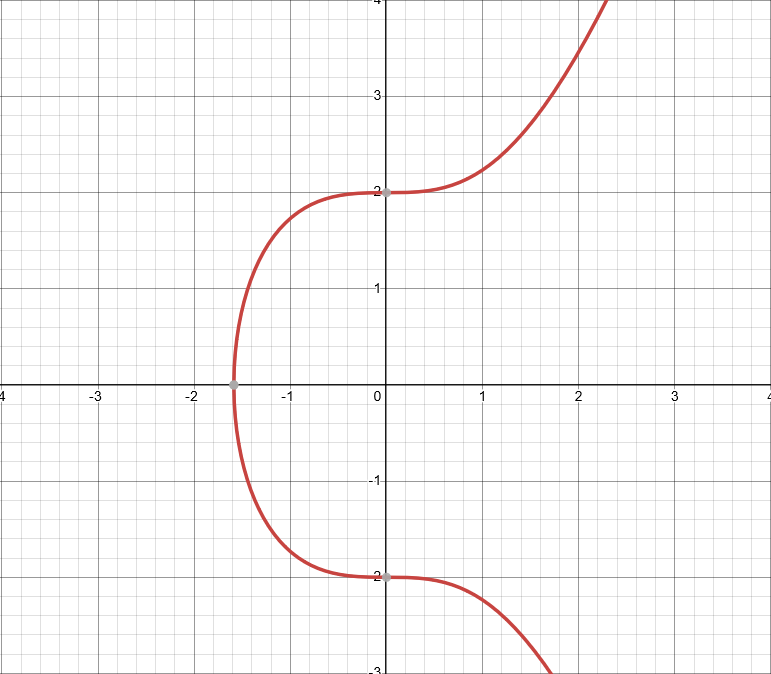
\includegraphics[width=0.5\linewidth]{BLS12-381curve.png}
\caption{BLS12-381 curve}
\label{Fig: BLS12-381}
\end{figure}




\subsection{About BLS12-381}

\subsubsection{History}

BLS12-381 was was designed by Sean Bowe in 2017. It was first used for an upgrade to \gls{Zcash protocol}. The curve is a pairing-friendly curve, which makes it efficient for digital signatures. In the draft of \gls{IETF} is BLS12-381 included with recommended parameters for a good security. \newline
It's naming comes from the family of curves described by Barreto, Lynn and Scott (BLS). The 12 is the embedding degree of the curve. The embedding degree will be discussed later on. The 381 is the number of bits needed to represent coordinates on the curve. This is also known as the size of the field modulus \textit{q}. These coordinates come from a finite field that has a prime order. This prime order has, in our case, the prime number \textit{q} which length is 381 bits. \cite{snark-curve-blog}

\subsubsection{Curve Equation And Parameters}
In the following section there will be no specific explanation of the mathematics used for the parameters. The equation for the BLS12-381 curve is: \\
\begin{center}
 \(y^2=x^3+4\). \\
\end{center}
For cryptographic purposes, the field \(F_q\) has to be extend to \(F_{q^2}\). By this extension the curve will change, adapting a new equation for the curve in \(F_{q^2}\):
\begin{center}
    \(y^2 = x^3 + 4(1+i)\)
\end{center}
It is important by the parametrization to optimize the pairing performance by choosing a parametrization with a low Hamming Weight. Essential are the base field modulus \textit{q} and the subgroup order \textit{r}. \\
In the BLS12-381 we have some parameters we have to set. But luckily there are some suggestions in the draft of the \gls{IETF} \cite{pairing-friendly-curves-website} to use for achieving a certain security level. \\
According to the \gls{IETF} draft \textbf{Pairing-Friendly Curves draft-yonezawa-pairing-friendly-curves-02} \cite{pairing-friendly-curves-website} BLS12-381 does not achieve 128 bits of security, so we regard it as an "optimistic" parameter. \\
We won't calculate new parameters because the goal of this document is to understand the theory behind the BBS signature scheme and implement a Java library. The BLS12-381 curve will only be handled theoretically.

In the BLS12-381 we have some parameters. But luckily there are some suggestions in the draft of the \gls{IETF} to use for achieving a certain security level. \\
We have the parameter \textbf{\textit{r}} which stands for the subgroup size in bits.


\subsubsection{Field Extensions}
Elliptic curves are defined over a field \textit{K} and describes points in \(K^2\).
field extensions are fundamental to elliptic curve pairings. The reason field extensions are important in pairing-friendly elliptic curves is that the target group \(G_T\) of the pairing is typically a group of order \textit{n} in a field extension \(F_{q^k}\) of the field \(F_q\) over which the elliptic curve is defined. For many cryptographic applications, this extension degree \textit{k} is crucial, as the efficiency and security of the system can depend on it. \\
In BLS12-381 we make a field extension from \(F_q\) to \(F_{q^{12}}\) what means the twelfth extension of \(F_q\). In the field \(F_{q^{12}}\) we find our group \(G_T\). \cite{bls12-381-hackmd}

\subsubsection{Curve}
In BLS12-381 we deal with two curves, one in the \(F_q\) field and the other in the extended \(F_{q^{12}}\) field. \\
The first curve is a simple curve in the \(F_q\) field. It consists of integers modulus \textit{q} that solve the equation \(y^2 = x^3 + 4\) for parameters \textit{x} and \textit{y}. The integers of \textit{x} and \textit{y} are each less than \textit{q}. The name of this curve is \(E(F_q)\). \\
The second curve is over the extension from \(F_q\) to \(F_{q^2}\). The equation for this curve is \(y^2 = x^3 + 4(1+i)\). This equation contains complex numbers, which will not be explained, but are crucial for the field \(F_{q^2}\). The second curve is named \(E'(F_{q^2})\). Doing arithmetic in \(F_{q^{12}}\) is extremely complicated and inefficient. That's because we're using a twist. The twist consists of a coordinate transformation from the \(F_{q^{12}}\) field into a lower degree field which still has an subgroup of order \textit{r}. The BLS12-381 has a "sextic twist", which means that it reduces the degree of the extension field by the factor six. That said, we have our \(G_2\) in a field of \(F_{q^2}\) instead of \(F_{q^{12}}\) which facilitates the calculations and enhances the efficiency of the BLS12-381 curve. \break
Our two groups we will be using are: \\
\begin{center}
\begin{itemize}
    \item \(G_1 \subset E(F_q)\) where \(E : y^2 = x^3 + 4\)
    \item \(G_2 \subset E'(F_{q^2})\) where \(E' : y^2 = x^3 + 4(1+i)\)
\end{itemize}
\end{center}


These two groups are used for a pairing \textit{e}. We have a point \(P \in G_1 \subset E(F_q) \) and a point \(Q \in G_2 \subset E'(F_{q^2}\). With \textit{P} and \textit{Q} we calculate a group operation which outputs a point from \(G_T \subset F_{q^{12}}\). The pairing \textit{e} is defined as \(e : G_1 \times G_2 \xrightarrow{} G_T\). \cite{bls12-381-hackmd}

\subsubsection{Embedding Degree}
The embedding degree of an elliptic curve is defined as the smallest positive integer such that \textit{r} (subgroup size) divides the number \((q^k -1)\). In the BLS12-381 curve k is 12, so \textit{r} is a factor of \((q^{12} - 1)\) but not of any lower power. \\
The embedding degree has an impact on security and efficiency. The higher the embedding degree the harder the discrete logarithm problem to solve \(G_T\). But the higher the embedding degree the more inefficient the calculations. So you have to find a embedding degree that fits the security without hurting the efficiency. \cite{bls12-381-hackmd}

\subsubsection{Cofactor}
The cofactors of the groups \(G_1\) and \(G_2\) are relevant for mapping the hashed message to a point into the respective subgroup \(G_1\) or \(G_2\). The cofactor is also used to find generators of the groups by scaling the smallest valid \textit{x}-coordinate and \textit{y}-coordinate, so the result is not the point at infinity. \cite{bls12-381-hackmd}

\subsection{Calculus in BLS12-381}
\subsubsection{Point Operations}
The primary calculus on the BLS12-381 involves point addition and point multiplication. These operations are not the usual addition and multiplication we know from arithmetic but are defined geometrically. For instance, point addition involves finding the line that intersects two points on the curve and then finding the third intersection point. Another operation is the point doubling. This simply adds the point to itself.
\begin{center}
  Point negation: \\
  \((x , -y)  = -(x , y) \) \\
  \vspace{5mm} 
  Point addition: \\
  \(\lambda = \frac{y_q - y_p}{x_q - x_p}\) \\
  \(x_r = \lambda ^2 - x_p - x_q\) \\
  \(y_r = \lambda(x_p - x_r) - y_p\) \\
  \vspace{5mm}
  Point doubling: \\
  \(\lambda = \frac{3{x_p}^2 + a}{2y_p}\)
\end{center}



\subsubsection{Scalar Multiplication}
The scalar multiplication of a point is a key operation in ECC and involves multiplying a point on the curve by a scalar. The scalar multiplication is the basic operation of points on the elliptic curve for the use in cryptography. The point is multiplied by itself. This operation is fundamental for key generation and encryption in ECC-based systems. To correclty calculate the scalar multiplication, the square and multiply method was used.
Formula

\subsubsection{Curve Calculations}
As we are doing a coordinate transformation, the \(E(F_q)\) has the familiar cartesian coordinates, but in \(E'(F_{q^2}\) the coordinates are polynomials consisting of coordinates from the field \(F_q\). This makes the calculation in the field \(F_{q^2}\) more inefficient for the curve calculations compared to the calculations in \(F_q\). 
A x-coordinate from \(E(F_q)\) is a number in the field \(F_q\). For \(E'(F_{q^2})\) it is a polynomial in the form of \(x'_0 + x'_1 * u\) for the x-coordinate. It is equivalent for the y-coordinate in \(E'(F_{q^2})\). For the calculations in \(F_{q^2}\) it is important to use the polynomial calculation for negate, add, multiply and inverting the polynomials.
For the elliptic curve point operation, the standard formulas are used, while using polynomials for the x and y values.
\begin{figure}[H]
    \centering
    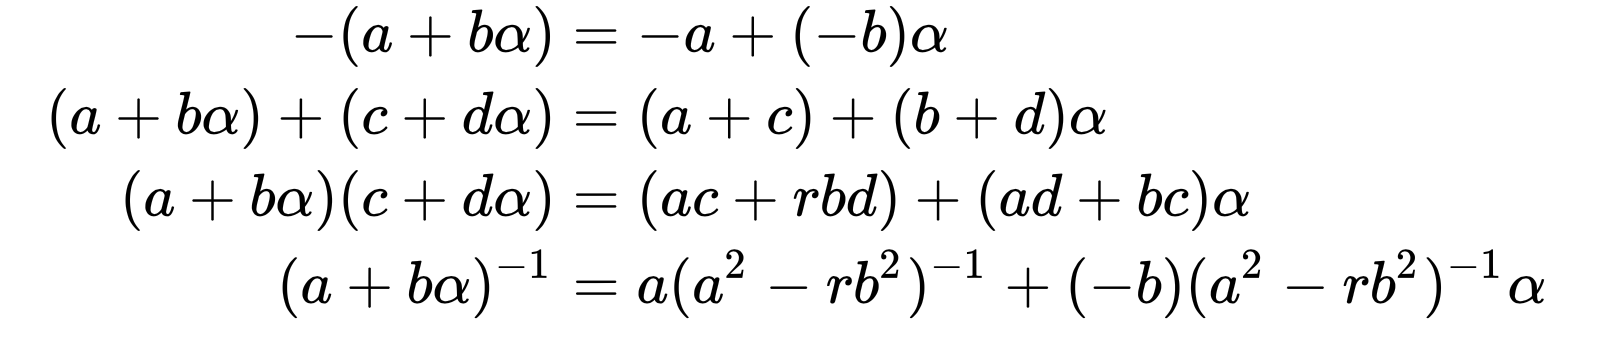
\includegraphics[width=0.5\linewidth]{polynomial_calc.png}
    \caption{Polynomial calculations}
    \label{Fig: polynomial calculations}
\end{figure}

\subsection{BLS12-381 Application}

In this section it'll be explained how the BLS12-381 is used for signing.

\subsubsection{Public And Private Keys}
For choosing the keys, it is first determined if group \(G_1\) or \(G_2\) is used for the keys. \(G_1\) is normally used for the key generation because \(G_1\) has smaller points and is faster than \(G_2\) which has large points and is slower. Interchanging the groups will affect the execution speed and the storage for the keys.\\
The secret key is a randomly chosen number between 1 and \textit{r-1} inclusive. The secret key is abbreviated by \textit{sk}. The public key is calculated with the equation \(pk = [sk]g_1\). \textit{pk} stands for public key and \(g_1\) stands for the generator of group \(G_1\). \cite{bls12-381-hackmd}

\subsubsection{Signing}
As \(G_1\) is used for the keys, \(G_2\) is used for signing a message \textit{m}. Firstly a mapping for \textit{m} to a point in the group \(G_2\) is done. It is done with the algorithm of "hash-and-check". \\
\begin{center}
\textbf{hahs-and-check}
\begin{enumerate}
    \item Hash message to an integer modulo \textit{q}.
    \item Enter the integer for coordinate \textit{x} and check if it has a coordinate \textit{y}. If not, add one and repeat this step.
    \item When \textit{y} coordinate is found, multiply by the \(G_2\) cofactor to convert it to a point in \(G_2\).
\end{enumerate}
\end{center}
After having found hashed message \textit{H(m)}, the signing is done by calculating \(\sigma = [sk]H(m)\). \cite{bls12-381-hackmd}

\subsubsection{Verification}
The verification is the part where pairing is used to verify the signature. It verifies if the sk is the corresponding to pk. The signature is valid if \(e(g_1,\sigma)= e(pk,H(m))\). \\
This can be verified easily with the properties of pairings:
\begin{center}
    \(e(pk,H(m)) = e([sk]g_1,H(m))= e(g_1,H(m))^{(sk)} = e(g_1,[sk]H(m)) = e(g_1,\sigma)\)
\end{center}
\cite{bls12-381-hackmd}


\section{Implementation}
The main Task of our Project, was to implement the pseudocode from the draft in Java as a library.
 
\subsection{Crypto Libraries}
A big part of the implementation is the chosen crypto library. Our part of the implementation is only focused on core BBS functionalities.
At the start of our implementation phase we had two libraries to choose from:
\href{https://github.com/herumi/mcl}{MCL} and \href{https://github.com/relic-toolkit/relic}{RELIC}
We choose to work with MCL for 2 reasons:
1. It's easier to use with Java, with its pre-generated JNI (Java native interface)
2. The pre-existing wrapper from Mr. Rolf Haenni made it easier to work with. \cite{mcl-github}
 
Starting in 2024, Mr. Rolf Haenni finished the first version of his crypto library, implemented in Java.
With that release we switched to that Library, which was further developed in the coming weeks.
 
\subsection{Java Implementation}
The first version of the implementation was just a proof of concept, if it was possible to implement the code in Java.
After confirming that everything works, the next part was to clean up the code and make it look the same as the pseudo code in the draft.
For that we created our own types, Scalar and OctetString, which are named in the draft.
With that we updated our implementation to look as close as possible to the draft.
After checking that this works to, we made the last step.
First we switched over to Mr. Haenni's crypto library.
Then we refactored the code into different classes, for better code quality.
Lastly we implemented the Test Vectors mentioned in the draft.

\section{Conclusion}
The conclusion of the Project 2 module is split in different subsections for a better separation of the conclusions to each topic. 

\subsection{Sub-tasks}
The research for BBS signature scheme wasn't easy. As it is a new cryptographic signature scheme there weren't many information about it. 
We had to read through all the scientific papers we found to decide which one is the suited for us. Some of them were to advanced for us to understand it and we had to discard them from our source of information. \\
For all the following topics it wasn't difficult at all finding some good papers on our level of knowledge to understand them. We also used slides from previous visited modules for the refresh of the topic elliptic curves.
Despite the interesting topic of elliptic curve pairings, we were not ready yet to understand the mathematics of pairings and only learned about what they are for and where they are used in \gls{BBS}. \\

\subsection{Main Task}
The most annoying thing about the implementation of \gls{BBS} was the constant change in the IETF draft and the mistakes we found by reading it. For the mistakes we made issues in the draft to alert the IETF that they have some mistakes in the pseudo code or in the text of the draft. Implementing the pseudo code wasn't a big hurdle but sometimes it got tricky. First we used the primitive type of byte arrays (byte []). After showing the code to our professors they recommended us to make our own type. So we made the type OctetString like in the pseudo code. 


\subsection{Project 2 Module}
The Project 2 module was a very nice experience for the both of us. It was a good preparation for the bachelor thesis and a good way to make a preparatory work to use it later. Having a project in a team with two students who work was really a challenge. Deciding when to meet for discussing the project or even the meeting with our professors. The project was bigger and harder than we thought but after some time we got used to invest several hours a week for this project.

\section*{Acknowledgements}
We would like to express our gratitude to our supervising professors Prof. Dr. Rolf Haenni and Prof. Dr. Reto Koenig. Thank you for your expertise, insight and commitment to ensuring the accuracy and clarity of this project. \\
Special thanks go to Prof. Dr. Rolf Haenni for implementing and giving us access to his personal library and adapt it to our code. \\
We also would like to acknowledge the support of Prof. Dr. Annett Laube. \newpage

\clearpage
\printglossaries
\printbibliography


\end{document}